\chapter{Lec 03 - Informed Search}
\section{Problem Solving: Informed Search}
The \textbf{Informed Search} strategy exploits a priori information on the problem to be solved to perform the search. The general approach we consider is called best-first search,  in which a node is selected for expansion based on an evaluation function, $f(n)$. The evaluation function is constructed as an estimate of “desirability”, so the node with the highest desirability is expanded first. Then, the frontier can be implemented as a queue sorted in decreasing order of desirability.
\newline\newline
The choice of $f$ determines the search strategy. Most best-first algorithms include as a component of $f$ a heuristic function, denoted $h(n)$.
\[h(n) =  \textit{estimate of cost from n to the closest goal}\]
Heuristic functions are the most common form in which additional knowledge of the problem is imparted to the search algorithm.\newline\newline
Special cases of best-first algorithms are:
\begin{itemize}
    \item Greedy search
    \item A* search
\end{itemize}

\section{Greedy search}
Greedy best-first search tries to expand the node that is closest to the goal, on the grounds that this is likely to lead to a solution quickly. Thus, it evaluates nodes by using just the heuristic function; that is, $f(n) = h(n)$.\newline\newline
In the Romania route-finding problem the heuristic function can be defined as the straight-line distance between a city and Bucharest.
\[h_{SLD}(n) =  \textit{straight-line distance from n to Bucharest}\]
\begin{center}
    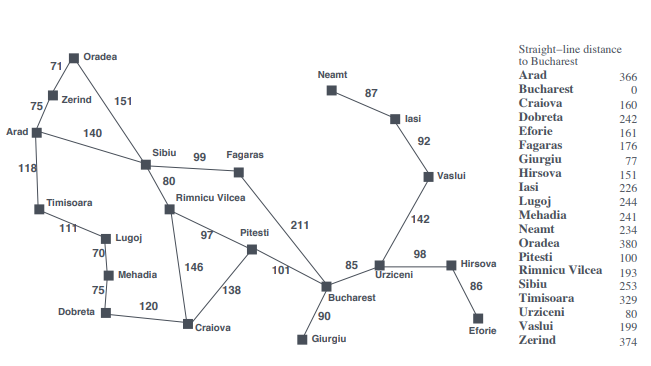
\includegraphics[]{images/heuristic.png}
    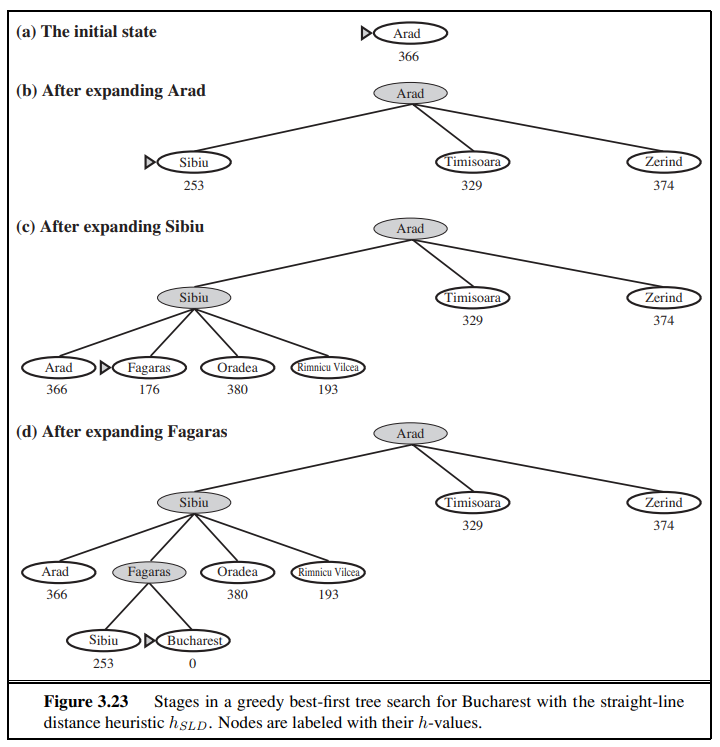
\includegraphics[]{images/greedy-approach.png}
\end{center}
The evaluation of the greedy best-first tree search is the following:
\begin{itemize}
    \item \textbf{Complete:} The algorithm is not complete; in fact, it can be stuck in loops (e.g. $In(Iasi) \rightarrow In(Neamt) \rightarrow In(Iasi) \rightarrow In(Neamt) \rightarrow$).

    \item \textbf{Time:} The worst-case time and space complexity for the tree version is $O(b^m)$,  where $m$ is the maximum depth of the search space. With a good heuristic function, however, the complexity can be reduced substantially.

    \item \textbf{Space:} $O(b^m)$ because it keeps all nodes in memory.

    \item \textbf{Optimal:} It's not optimal since it is not complete.
\end{itemize}
The graph search version is complete in finite spaces, but not in infinite ones.

\section{A* search}
The most widely known form of best-first search is called \textbf{A* search}. It evaluates nodes by combining $g(n)$, the cost to reach the node $n$, and $h(n)$, the cost to get from $n$ to the goal:
\[f(n) = g(n) + h(n)\]
Since $g(n)$ gives the path cost from the start node to node $n$, and $h(n)$ is the estimated cost of the cheapest path from $n$ to the goal, we have
\[f(n) = \textit{estimated cost of the cheapest solution through n}\]
Thus, if we are trying to find the cheapest solution, a reasonable thing to try first is the node with the lowest value of $g(n) + h(n)$.\newline\newline
A* search uses an \textbf{admissible heuristic}, that is, it never overestimates the cost to reach the goal; $h(n) \leq h^*(n)$, where $h^*(n)$ is the true cost from $n$. It also requires $h(n) \geq 0$, so $h(G) = 0$ for any goal $G$.
\begin{center}
    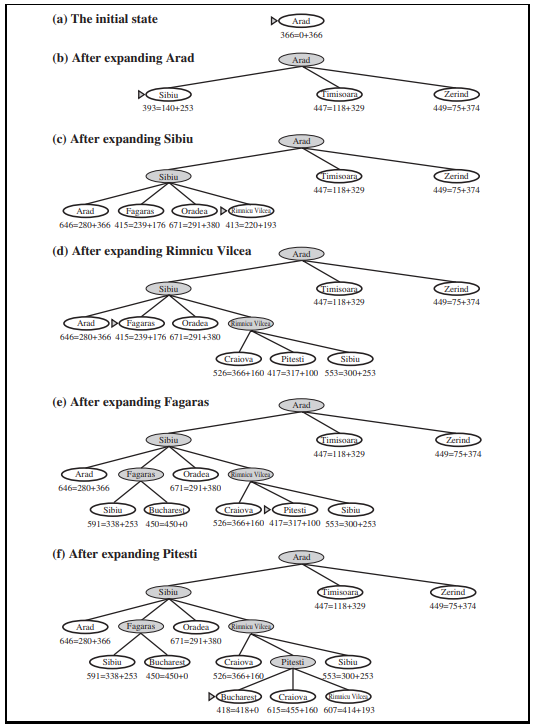
\includegraphics[]{images/A-search.png}
\end{center}
\textbf{Theorem:} the tree-search version of A* is optimal if $h(n)$ is admissible.\newline\newline
\textbf{Proof:}
Suppose some suboptimal goal $G_2$ has been generated and is in the queue. Let $n$ be an unexpanded node on a shortest path to an optimal goal $G$.
\[
\begin{split}
    f(G_2) & = g(G_2)\,\, \text{since $h(G_2) = 0$}\\
    & > g(G) \,\, \text{since $G_2$ is suboptimal}\\
    & \geq f(n) \,\, \text{since $h$ is admissible}
\end{split}
\]
Since $f(G_2) > f(n)$, A* will never select $G_2$ for expansion.
\newline\newline
The property above does not work for the graph-search version of A*. This is because there is a risk of discarding a repeated occurrence of a state that
is on an optimal path (since graph-search does not visit an already visited node).\newline\newline
A solution to this problem is to use \textbf{consistent} heuristics: A heuristic $h(n)$ is consistent if, for every node $n$ and every successor $n'$ of $n$ generated by any action $a$, the estimated cost of reaching the goal from $n$ is no greater than the step cost of getting to $n'$ plus the estimated cost of reaching the goal from $n'$:
\[h(n) \leq c(n, a, n') + h(n')\]
This is a form of the general \textbf{triangle inequality}, which stipulates that each side of a triangle cannot be longer than the sum of the other two sides. Here, the triangle is formed by $n$, $n'$, and the goal $G_n$ closest to $n$.
\newline\newline
\textbf{Theorem:} e the graph-search version of A* is optimal if $h(n)$ is \textbf{consistent}.\newline\newline
\textbf{Proof:} if $h$ is consistent, we have:
\begin{center}
    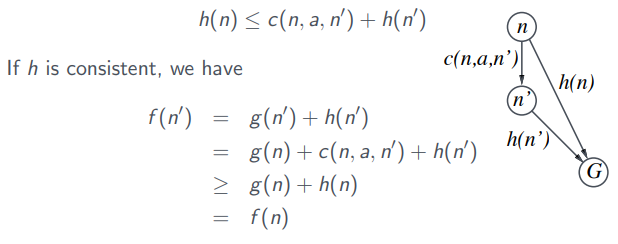
\includegraphics[]{images/consistency.png}
\end{center}
Therefore, $f(n)$ is non-decreasing along any path.\newline\newline
From the preceding observation, it follows that the sequence of nodes expanded by A* using GRAPH-SEARCH is in non-decreasing order of $f(n)$.  Hence, the first goal node selected for expansion must be an optimal solution because $f$ is the true cost for goal nodes (which have $h = 0$) and all later goal nodes will be at least as expensive.\newline\newline
The fact that f-costs are nondecreasing along any path also means that we can draw \textbf{contours} in the state space, just like the contours in a topographic map.
\begin{center}
    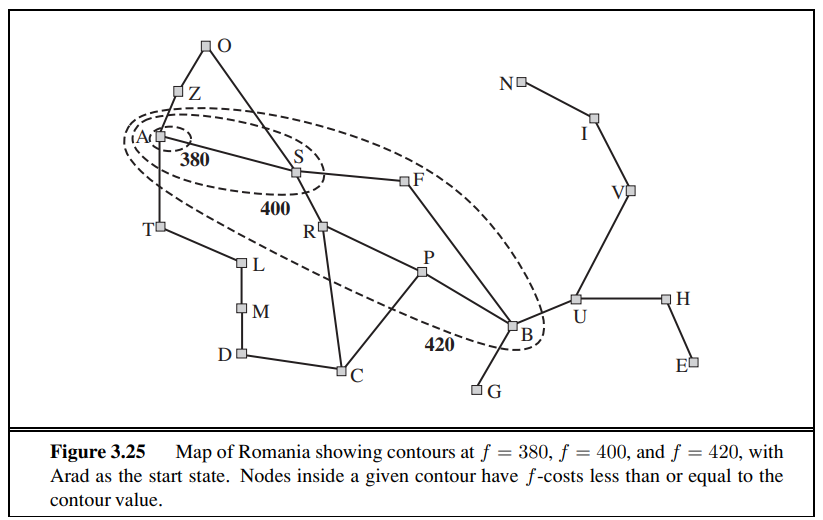
\includegraphics[scale=0.8]{images/topological map.png}
\end{center}
Properties of A*:
\begin{itemize}
    \item \textbf{Complete:} Yes, unless there are infinitely many nodes with $f \leq f(G)$.

    \item \textbf{Time:} Exponential in [relative error in $h \times$ length of solution].

    \item \textbf{Space:} Keeps all nodes in memory.

    \item \textbf{Optimal:} Yes (it follows from the theorems). It expands all nodes with $f(n) < C^*$, where $C^*$ is is the cost of the optimal solution path. It might then expand some of the nodes right on the “goal contour” (where $f(n) = C^*$) before selecting a goal node. It expands no nodes with $f(n) > C^*$
\end{itemize}
A* is not only optimal: no other optimal algorithm is guaranteed to expand fewer nodes than A* (except possibly through tie-breaking among nodes with $f(n) = C^*$). In fact, any algorithm that does not expand all nodes with $f(n) < C^*$ runs the risk of missing the optimal solution.

\section{Iterative Deepening A*}
A* is exponential in space and therefore not applicable to many real-world problems. The main problem is that the frontier grows exponential in size even if
most of the nodes will never be extracted ($f(n) > C^*$). In order to reduce the use of memory of A* we can exploit the same idea behind Iterative Deepening Search. \newline\newline
The idea is to iteratively increase the $f$-value, just as Iterative Deepening Search increases the depth level. However, the $f$-value is a real number and cannot just be incremented by 1. Therefore, at iteration $i+1$, we can  use the best $f$-value of nodes that were not inserted in the frontier at iteration $i$.
\newline\newline
This procedure is called Iterative Deepening A* and it works as follows:
\begin{enumerate}
    \item a \textbf{cutoff} value for $f$ is defined (initially equal to 0)

    \item during an iteration, a node $n$ is \textbf{not} inserted in the frontier if its $f$-value is larger than the cutoff value ($f(n) > cutoff$).

    \item when the queue is empty (and no goal found) a new iteration is started with a new cutoff value.

    \item the new cutoff value is given by the minimum $f$-value among all the nodes not inserted in the queue.
\end{enumerate}

